\documentclass[a4paper,12pt]{mythesisclass}
% Your custom document content starts here
% (Title page, abstract, chapters, sections, figures, tables, references, etc.)

\begin{document}
	% Cover Page
	\begin{titlepage}
		\begin{center}
			% University Logo
			
\includegraphics[width=5cm]{qm_logo.png} % Replace with actual path
			
			\vspace{1.5cm}
			
			\Large\textbf{Leveraging Transfer Learning and Multi-AI Agents for the Design of Self-Assembled Monolayer Molecules} % Title Placeholder
			
			\vspace{1cm}
			
			\Large
			By \\
			\textbf{Harrison-Li} % Name Placeholder
			
			\vspace{1cm}
			
			Materials Science and Engineering \\
			
			\vspace{0.5cm}
			
			QXU6021 Final Year Project
			
			\vspace{1cm}
			
			\textbf{Supervisor} 
			\underline{Prof. ****} % Placeholder for supervisor name
			
			\vspace{0.5cm}
			\textbf{Advisor}
			\underline{Prof. ****} % Placeholder for supervisor name
			
			\textbf{Graduation Date}
			\underline{June 2025}
			
			\vfill
			
			{\large Queen Mary University of London \\ QMUL Engineering School, NWPU}
			
		\end{center}
	\end{titlepage}
	\newpage
	\begin{titlepage}
		% University logo and title
		\begin{center}
			
\includegraphics[scale=0.8]{NPU_logo.png} % Replace with your logo if needed
			\\
			\LARGE\textbf{Undergraduate Graduation}\\
			\LARGE\textbf{Design (Thesis)}
		\end{center}
		
		\noindent Title
		
		\begin{center}\vspace{-5mm}
			Leveraging Transfer Learning and Multi-AI Agents for the Design of\\
			\rule{0.8\linewidth}{0.5pt}\\
			Self-Assembled Monolayer Molecules\\
			\rule{0.8\linewidth}{0.5pt}
		\end{center}
		\noindent Major
		\begin{center}\vspace{-5mm}
			Materials Science and Engineering\\
			\rule{0.8\linewidth}{0.5pt}
		\end{center}

		\noindent Name
		\begin{center}\vspace{-5mm}
			Harrison-Li\\
			\rule{0.7\linewidth}{0.5pt}
		\end{center}
        
		\noindent Supervisor
		\begin{center}\vspace{-5mm}
			Prof. ****\\ % 替换星号为supervisor名字
			\noindent\rule{0.7\linewidth}{0.5pt}
		\end{center}
        
		\noindent Advisor
		\begin{center}\vspace{-5mm}
			Prof. ****\\ % 替换星号为advisor名字
			\noindent\rule{0.7\linewidth}{0.5pt}
		\end{center}
        
		\noindent Graduation Date
		\begin{center}\vspace{-5mm}
			June 2025\\
			\noindent\rule{0.7\linewidth}{0.5pt}
		\end{center}
		
	\end{titlepage}
	\newpage
	\begin{titlepage}
		\begin{center}
			\textbf{QMUL ENGINEERING SCHOOL OF NPU}
			
			\vspace{1.5em}
			
			\textbf{MATERIALS SCIENCE AND ENGINEERING}
			
			\vspace{1.5em}
			
			\textbf{FINAL YEAR PROJECT}\\
			\textbf{QXU6021}\\
			\textbf{June 2025}
			
			\vspace{2em}
			
			\textbf{DECLARATION}
		\end{center}
		
		\vspace{2em}
		
		\noindent This report entitled
		
		\vspace{1em}
		
		\begin{center}
			\textbf{Leveraging Transfer Learning and Multi-AI Agents for the Design of Self-Assembled Monolayer Molecules}
		\end{center}
		
		\vspace{1em}
		
		\noindent was composed by me and is based on my own work. Where the work of the others has been used, it is fully acknowledged in the text and in captions to table illustrations. This report has not been submitted for any other qualification. I also declare that all information in this thesis have been acquired and presented in accordance with academic rules and ethical conduct of QMES. The thesis, or part of it, has not been generated using any artificial intelligence editing tools. I am fully aware that a gross academic misconduct would invalidate my bachelor’s degree.
		
		\vspace{1em}
		
		\noindent \textbf{Name} \hspace{1em} \textbf{Harrisonli}
		\vspace{1cm}
		
		\noindent \textbf{Signature} \hspace{1em}
        \vspace{1cm}
		
		\noindent \textbf{Date}  \hspace{1cm} May 6, 2025
		
	\end{titlepage}
\tableofcontents
\chapter{Introduction}
\section{Motivation}
组合图
\begin{figure}[H]
	\centering
    \textbf{\sidesubfloat[]{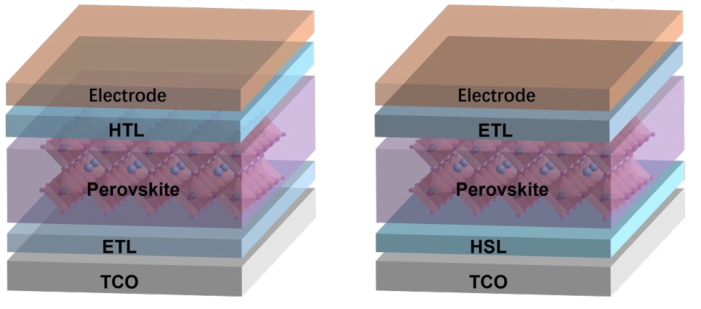
\includegraphics[width=0.55\linewidth]{figures/PSC_schematic.pdf}}}
	\textbf{\sidesubfloat[]{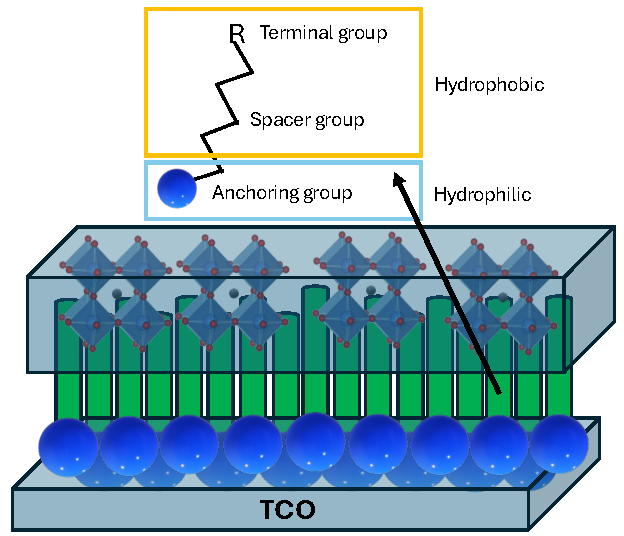
\includegraphics[width=0.34\linewidth]{figures/SAMs_structure.pdf}}}\vfill
    \textbf{\sidesubfloat[]{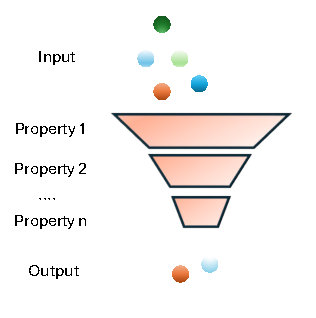
\includegraphics[width=0.35\textwidth]{figures/filter.pdf}}}
	\textbf{\sidesubfloat[]{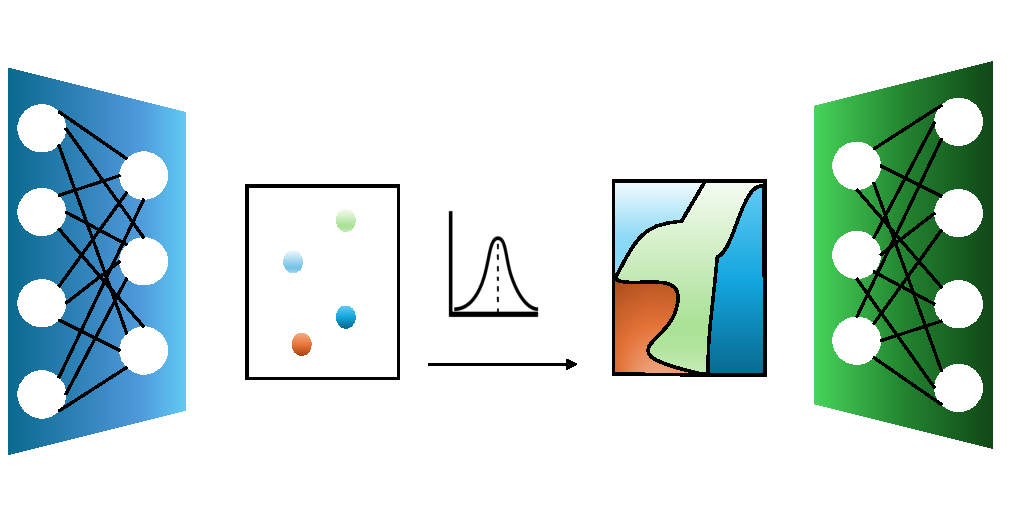
\includegraphics[width=0.55\textwidth]{figures/inverse_design.pdf}}}		
	\caption{\textbf{(a)} Device structure of regular PSC (left) and inverted PSC (right).\cite{li2024self} \textbf{(b)} Schematic of self-assembled-monolayers. \textbf{(c)}  Materials design via screening. \textbf{(d)} Inverse design via generative models.}
	\label{background}
	\end{figure}
\section{Current state of art}


\chapter{Method}

\chapter{Result and Discussion}
\subsection{组合图}



\begin{table}[t]
    \caption{\raggedright  Performance Metrics of Target Property Molecular Generation}\label{prop_performance}
    \resizebox{0.7\textwidth}{!}{%	
		\begin{tabular}{@{}l l r r r@{}}
			\toprule
			\rowcolor[HTML]{E0E0E0} 
			\textbf{Property} & 
            \textbf{prop1} & 
			\textbf{prop2} & 
			\textbf{prop3} \\
			\midrule
            prop1 (3.5) & 0.967 & 0.635 & 0.948  \\ 
            prop2, prop3 (15,250) & 0.9 & 0.99 & 5  \\
			prop5, prop6 (1,2) & 1 & 0.2 & 0.996  \\
			\bottomrule
		\end{tabular}
	}
\end{table}

\subsubsection{三线表}
三线表参考表\ref{table3}
\begin{table}[H]
    \fontsize{10.5bp}{1.25}
    \caption{表格标题}
    % \setlength{\abovecaptionskip}{0.2cm}  %调整标题与图距离
    % \setlength{\belowcaptionskip}{0.2cm} %调整标题与下文距离
    \centering\label{table3}
    % \vspace{-0.5em}	
    \begin{tabular}{cccc}
        \toprule[1.5pt]
        方法       & A算法 & B算法 & C算法 \\
        \toprule[1.5pt]
        误差/dB    & 0.86  & 1.02  & 0.69  \\
        计算时间/s & 25    & 25    & 27    \\
        \toprule[1.5pt]
    \end{tabular}
\end{table}
\chapter{Conclusion}

\bibliography{reference}
\chapter*{Appendices}

\chapter*{Acknowledgment}
谢天谢地谢鬼神


\end{document}